\documentclass{article}
\usepackage{graphicx}
\usepackage{subcaption}
\usepackage[a4paper, total={16cm, 24cm}]{geometry}
\usepackage{xspace}
\usepackage[hidelinks]{hyperref}
\usepackage{color}
\usepackage{fancyvrb}
\usepackage{comment}
\usepackage{pdflscape}
\newcommand{\shiv}{\c{shiver}\xspace}
\newcommand{\sac}{\c{shiver\char`_align\char`_contigs.sh}\xspace}
\newcommand{\smr}{\c{shiver\char`_map\char`_reads.sh}\xspace}
\let\c\texttt
\newcommand{\www}{\color{blue} \underline}
\setcounter{tocdepth}{2}
\setcounter{secnumdepth}{2}

\title{\shiv\\available from \href{https://github.com/ChrisHIV/shiver}{\www{https://github.com/ChrisHIV/shiver}}}
\date{This manual last updated \today}
\author{By Chris Wymant}

\begin{document}
\maketitle


\begin{figure}[!h]
\centering
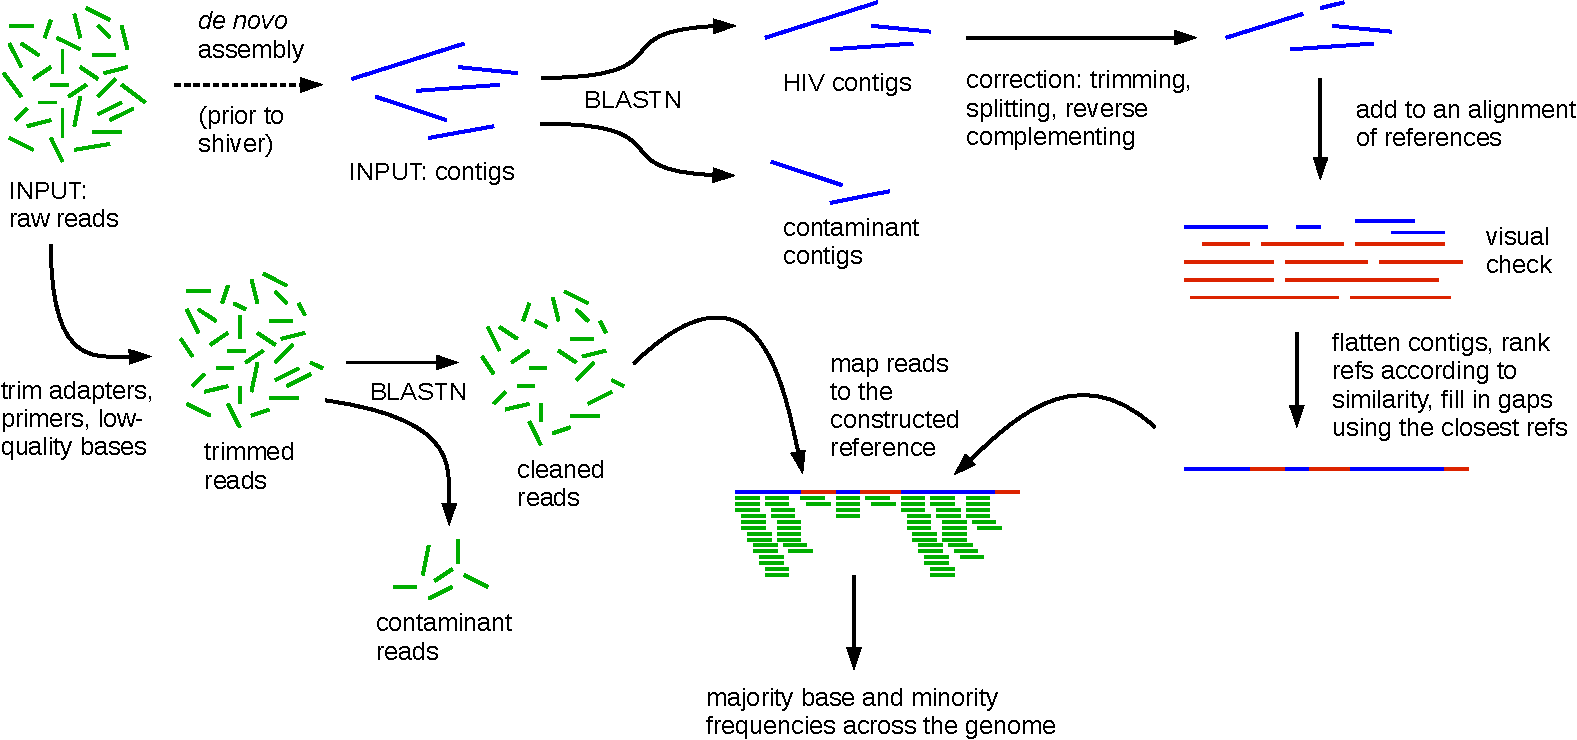
\includegraphics[width=0.95\textwidth]{AssemblyPipelineDiagram_ForPaper.pdf}
\end{figure}


\shiv is a tool for mapping reads (fragments of genetic sequence) to a custom reference sequence constructed using contigs, in order to minimise the biased loss of information that occurs from mapping to a reference that differs from the sample.
From the mapped reads, base frequencies are quantified, and a consensus sequence is called.
\shiv was designed for HIV but has broader applicability; if you are using it for sequence data from organism X instead of HIV, mentally replace {\it HIV} by {\it X} when reading this manual.

The method and its performance are discussed \href{https://doi.org/10.1093/ve/vey007}{\www{here}}; please cite this if you find \shiv helpful.
If you use \shiv, please cite the publications of its dependencies: \c{SAMtools}~\cite{Li08062009}, \c{MAFFT}~\cite{Katoh15072002}, \c{blast}~\cite{ALTSCHUL1990403}, \c{Biopython}~\cite{biopython}, \c{Trimmomatic}\cite{Bolger01082014} (only if you use \shiv's option to trim reads for adapters and quality), and \c{BWA}~\cite{doi:10.1093/bioinformatics/btp698} or \c{bowtie}~\cite{Langmead2009} (if you switched the default mapper from \c{smalt}, for which there is no publication to cite).
If you install \shiv using  \c{bioconda}, please cite \c{bioconda}~\cite{Gruning2018-fj}.
Details of these publications are in the file \c{CitationDetails.bib} in \shiv's \c{docs} subdirectory.
Finally don't forget to cite whatever method you use to assemble contigs as input for \shiv.

\shiv is run `through the command line' (or `in a terminal'), not by clicking on things in a graphical user interface.
If you don't know how to run programs from the command line, you need to learn that first\footnote{These resources were recommended by the organisers of the Wellcome Genome Campus' {\it Genomics and Clinical Virology} course: \href{http://rik.smith-unna.com/command_line_bootcamp}{\www{http://rik.smith-unna.com/command\_line\_bootcamp}},\\
\href{http://www.ee.surrey.ac.uk/Teaching/Unix}{\www{http://www.ee.surrey.ac.uk/Teaching/Unix}},\\
\href{http://swcarpentry.github.io/shell-novice/}{\www{http://swcarpentry.github.io/shell-novice/}}.}.

\shiv runs natively on Linux and Mac OS, but not Windows.
For guidance on installing \shiv, see the readme file that displays at the \href{https://github.com/ChrisHIV/shiver}{GitHub repository}.

If you have a problem getting the code to run or think you've found a bug, please create a \href{https://github.com/ChrisHIV/shiver/issues}{\www{\it New issue}} on the GitHub repository.

Throughout this manual, I'll assume your \shiv code lives in \c{\path{~}/shiver/}.
If you downloaded it somewhere else, e.g. \c{my/other/directory/shiver/}, simply replace every occurrence of \c{\path{~}/shiver/} in this manual by \c{my/other/directory/shiver/}; alternatively if you're feeling lazy, create a symbolic link to \c{my/other/directory/shiver}, call it \c{shiver}, and put it in your home directory.

By default, to run a \shiv command, you have to tell the command line where the binary/executable file for that command is found, i.e. including its path, e.g. \c{\path{~}/shiver/bin/shiver\char`_align\char`_contigs.sh}.
If you don't want to type the path every time -- you want to be able to just type \sac -- you need to add the directory containing the \shiv binary files (\c{\path{~}/shiver/bin}) to your \c{PATH} environmental variable.
Search on Google if you don't know how to do that.
{\bf Do not} add `\texttt{sh }' before a \shiv command -- this forces your operating system to interpret the code as shell language (it's actually bash) and will result in a strange error.

Throughout this manual, a \c{\$} character at the start of a line just indicates that what follows should be run from command line; you should be able to just copy and paste this into your terminal, then press enter to execute the command.
Don't include that initial \c{\$} character in what you copy and paste.
Be sure to highlight the whole command for copying and pasting.
If a command is split over multiple lines, you can copy all of them in one go then press enter.

\tableofcontents

\newpage
\section{Initialisation}
Before you begin processing a collection of samples there's an initialisation step: it should be run once only (i.e. not once for each sample).
It requires:
\begin{itemize}
\item A \shiv configuration file, in which you can specify parameters, options etc. and tell \shiv what commands to use to call external programs.
A configuration file with default values is provided in \c{\path{~}/shiver/bin/config.sh} (this file is not intended to be executed, only to be given as an argument for the other shiver binary files, but I put it in the \c{bin} directory for want of a better idea).
Here it is needed only to tell \shiv how to run the program \c{blast}; you can change your mind about all the pipeline parameters contained in this file later on.
The config file is discussed further in section \ref{sec:config}.  
\item An alignment of your choice of existing reference genomes (lots of which are available to download from the \href{http://www.hiv.lanl.gov/content/sequence/NEWALIGN/align.html}{\www{LANL HIV database}}) called \c{MyRefAlignment.fasta}, say.  
\item Fasta files containing the adapters and PCR primers used for sequencing, called \c{MyAdapters.fasta} and \c{MyPrimers.fasta}, say.
Adapters will be removed using Trimmomatic, and ``The naming of the various sequences within this file determines how they are used'' -- the Trimmomatic manual.
Adapter sequence is trimmed out of reads, wherever it is found; afterwards PCR primer sequences are trimmed when perfect matches to them are found at the end of a read.
\end{itemize}


Initialisation files will be put into a directory called \c{MyInitDir} if you run
\begin{Verbatim}[samepage=true]
$ ~/shiver/bin/shiver_init.sh  MyInitDir  config.sh  MyRefAlignment.fasta  \
  MyAdapters.fasta  MyPrimers.fasta
\end{Verbatim}
(remembering to skip that first \c{\$} character.)
You shouldn't touch \c{MyInitDir} or the files therein after running this command, or unknown bad things might happen.

After running that initialisation command (once only!), you can process any number of samples.
Sample processing writes and reads in again (many) files in the working directory, so {\bf it's very important work in a separate, empty directory for each sample you process}.
Otherwise you might overwrite existing files, or the files from processing one sample could interfere with the files from processing another sample.
There's an example of creating a new directory for each of a series of samples in section \ref{sec:scripting}.

\section{How to process a single sample} \label{sec:SingleSample}

The input for each sample is (1) reads, and (2) contigs that were assembled from those reads.
\begin{enumerate}
\item As of version 1.6.0, shiver can handle both {\it paired} reads (each fragment is sequenced forwards from one end and backwards from the other) and unpaired reads (one read is generated per fragment).
\begin{itemize}
\item If your data is paired reads, the forward read names must all end in ``/1'', the reverse read names must all end in ``/2'', and mates in a pair must match in what comes before this.
e.g. Forward read names might be {\it FirstReadName/1}, {\it SecondReadName/1}, $\ldots$ and reverse read names should then be {\it FirstReadName/2}, {\it SecondReadName/2}, $\ldots$ This is so \shiv knows how to pair the reads together.
\item If your data is unpaired reads, there are no restrictions on read names.
\end{itemize}
\item Our favourite assembler is IVA; it can be installed from \href{http://sanger-pathogens.github.io/iva/}{\www{here}} or run on a virtual machine \href{http://sanger-pathogens.github.io/pathogens-vm/}{\www{here}}, and the publication is \href{http://bioinformatics.oxfordjournals.org/content/early/2015/02/27/bioinformatics.btv120.abstract}{\www{here}}.
Say your forward reads are in \c{reads\char`_1.fastq.gz} and your reverse reads are in \c{reads\char`_2.fastq.gz}; assembling them into contigs is as simple as running
\begin{Verbatim}[samepage=true]
$ iva  -f  reads_1.fastq.gz  -r  reads_2.fastq.gz  MyOutputDirectory
\end{Verbatim}
though you should run \c{iva --help} to see the options, including specifying adapter and primer sequences to trim from the reads.
\shiv wants {\it all} contigs produced by assembly; if by curiosity you check what organisms the different contigs come from, do not remove non-HIV contigs.
These contaminant contigs (if present) are used to help remove contaminant reads.
\end{enumerate}

Processing a sample requires two commands.
If your contigs are in a file \c{contigs.fasta}, the first command is  
\begin{Verbatim}[samepage=true]
$ ~/shiver/bin/shiver_align_contigs.sh  MyInitDir  config.sh  contigs.fasta  SID
\end{Verbatim}
replacing \c{SID} (`sample ID') by a name used for labelling all output files for this sample.
This command will produce a file named \c{SID.blast} (detailing blast hits of your contigs to those existing references supplied for the initialisation).
Assuming at least one contig looks like HIV, \c{SID.blast} will not be empty (see section \ref{sec:ContiglessSamples} otherwise), and there will be another file called \c{SID\char`_raw\char`_wRefs.fasta} -- an alignment of the HIV contigs (i.e. those that have blast hits) to your input existing reference genomes.
In this alignment, nothing has been done to the contigs (hence the name {\it raw}).

\shiv decides that a contig needs correcting, if it
\begin{itemize}
 \item is not wholly spanned by a blast hit, suggesting that the ends are not genuine HIV and should be trimmed off;
 \item has two or more blast hits (ignoring hits wholly inside other hits), suggesting that it is chimeric/spliced -- erroneously connecting disconnected parts of the genome;
 \item has a blast hit in the opposite orientation to the reference, suggesting that that contig (or part of it) should be reverse complemented;
 \item contains an unrealistically large gap after alignment to the existing references, suggesting that it should be split into two separate contigs;
 \item overhangs the edge of the alignment of existing references (i.e. in the alignment the beginning of the contig is to the left of the beginning of all references, or the end of the contig is to the right of the end of all references).
\end{itemize}
Appropriate action is taken in each case -- trimming, cutting into pieces, and reverse-complementing as needed.
If any of these actions were needed for any of the contigs, an additional file \c{SID\char`_cut\char`_wRefs.fasta} will be produced, which contains all contigs after correction, aligned to the existing references.
We expect that \c{SID\char`_cut\char`_wRefs.fasta} (if it exists) is a better alignment than \c{SID\char`_raw\char`_wRefs.fasta}, but it's safer not to take this for granted, for example unusual indels can result in multiple blast hits.
Therefore both of these files should be inspected, the better one chosen, and edited if necessary; we go into a lot more detail about this in section \ref{sec:ContigAlnExamples}.

With an alignment of contigs you're happy with, say \c{SID\char`_cut\char`_wRefs.fasta}, and if your paired reads are in files \c{reads\char`_1.fastq.gz} and \c{reads\char`_2.fastq.gz}, run
\begin{Verbatim}[samepage=true]
$ ~/shiver/bin/shiver_map_reads.sh  MyInitDir  config.sh  contigs.fasta  SID  \
  SID.blast  SID_cut_wRefs.fasta  reads_1.fastq.gz  reads_2.fastq.gz
\end{Verbatim}
or if you have unpaired reads, replacing \c{reads\char`_1.fastq.gz reads\char`_2.fastq.gz} by your single file of reads.

\section{What output do I get?}

Output files include:
\begin{itemize}
\item \c{SID.bam}, \c{SID\char`_ref.fasta}: the bam file of mapped reads, and the reference sequence to which they were mapped.
\item \c{SID\char`_BaseFreqs.csv}: the frequencies of A, C, G, T, `-' for a deletion, and N for unknown, at each position in the genome.
\c{SID\char`_BaseFreqs\char`_ForGlobalAln.csv} is almost the same thing: it contains an extra column with a coordinate that can be used to compare different samples, at the cost of having to skip some rows for which this coordinate is ambiguous.
Specifically, the extra coordinate is position in the {\it global alignment} (see section~\ref{sec:GlobalAln}), and the rows that are skipped are positions where the reads had an insertion with respect to the mapping reference.
Positions where the mapping reference has an insertion with respect to the global alignment (i.e. where the contigs had an insertion with respect to the existing references you gave \shiv as input) are included at the appropriate position in this file, just with an undefined global coordinate.
\c{SID\char`_BaseFreqs\char`_WithHXB2.csv} is the same thing as \c{SID\char`_BaseFreqs\char`_ForGlobalAln.csv} but using the coordinates of the HXB2 sequence instead of the coordinates of the global alignment (this is only produced if the config file variable \c{GiveHXB2coords} is left at its default value of \c{true}; you'll certainly want to change this to \c{false} if you're using \shiv on non-HIV data).
\item \c{SID\char`_MinCov\char`_X\char`_Y.fasta}: the pairwise alignment of the consensus genome and the reference used for mapping.
In place of \c{X} and \c{Y} here you'll see the two coverage thresholds specified in \c{config.sh}: \c{X} is the minimum number of reads to call a base (if there are fewer than \c{X} reads we call \c{?} instead of a base), \c{Y} the minimum number to use upper case for the base (to signal increased confidence).
The mapping reference is included with the consensus here to give context to any \c{?} characters.
\item \c{SID\char`_MinCov\char`_X\char`_Y\char`_ForGlobalAln.fasta}, \c{SID\char`_coords.csv}: these files are useful when multiple samples are processed, so we postpone their explanation to section~\ref{sec:GlobalAln}.  
\item \c{SID\char`_InsertSizeCounts.csv}: the insert-size distribution.
\end{itemize}
If the config file variable \c{remap} is left at its default value of \c{true}, some of the files named above will have a second copy with \c{SID} replaced by \c{SID\char`_remap} in the file name.
These are the result of remapping to the consensus called from the first round of mapping.
The files \c{SID[something]} and \c{SID\char`_remap[something]} will likely be very similar, but the latter is expected to be slightly more accurate.
Files related to the global alignment do not have a remapped counterpart (see the final paragraph of section \ref{sec:GlobalAln} for the reason why).

Some files are not produced by default, but their production can be specified in \c{config.sh}:
\begin{itemize}
\item \c{SID\char`_PreMapping\char`_1.fastq}, \c{SID\char`_PreMapping\char`_2.fastq}.
These are produced if you change the value of the config file variable \c{KeepPreMappingReads} to \c{true}.
They are the reads after removal of (i) adapters, (ii) PCR primers, (iii) low-quality bases, and (iv) those reads suspected of being contamination based on blasting to the contaminant contigs.
This corresponds to the state of the reads right before the mapping step.
Note that not all of these reads will map, for example because the removal of suspected contaminant reads based on the contaminant contigs is not perfectly sensitive (some contaminant reads may not have been assembled into contigs).
So if what you're after is the fully processed reads with as many contaminant reads removed as possible (e.g. to upload to some public database), you don't want these files, you want the reads from the bam file.
(By default these files are produced, but with \c{temp\char`_} prepended to their names to indicate that you probably don't want to keep them.)
\item \c{SID\char`_MinCov\char`_X\char`_Y\char`_wContigs.fasta}.
This is produced if you change the value of the config file variable \c{AlignContigsToConsensus} to \c{true}.
It is an alignment of the consensus, the reference used for mapping, and all HIV contigs for this sample (as they were after any automatic cutting and any manual editing).
This is just for interest, to see how the contigs compare with the consensus.
\item \c{SID\char`_ContaminantReads.bam}.
This is produced if you change the value of the config file variable \c{MapContaminantReads} to \c{true}.
It is a bam file of only the contaminant reads mapped to the HIV reference; it shows you the contaminant reads that would have been in your bam file of genuine reads if you had turned off the contaminant-contig-based cleaning of reads.
\end{itemize}

Lots of intermediate/temporary files are produced during processing; these you probably don't want to keep.
By default their names all begin \c{temp\char`_} (you can change this in the config file if you really want).
If you
\begin{itemize}
\item chose a sample ID (for labelling output) that was not \c{temp} and did not begin with \c{temp\char`_}, and
\item ran \shiv from inside an empty directory as strongly advised, and 
\item are still inside the same directory where you ran \shiv, and
\item have not added any other files with names beginning \c{temp\char`_} since running \shiv,
\end{itemize}
then the command \c{rm temp\char`_*} will delete all and only the temporary files.
(Warning: the \c{rm} command irrecoverably deletes files, and the wildcard character \c{*} matches {\it anything}.
If you accidentally put a space between \c{temp\char`_} and \c{*}, the previous command would delete {\it all files} in the current directory.
If the \c{rm} command makes you nervous, you can delete files by selecting them in a graphical file explorer window and clicking delete (probably, depending on your operating system).)

\section{The config file} \label{sec:config}
In \c{config.sh} you can change pipeline parameters from their default values.
During development of \shiv, \c{config.sh} has often been updated (some new features required new parameters).
As this may happen again in the future, to make sure you keep any changes you've made to default values, I recommend the following: rename \c{config.sh} to \c{config\char`_original.sh}, make a second copy called \c{config\char`_MyChanges.sh}, leave the former untouched and change whatever you like in the latter.
Then when you update your \shiv code (by running \c{git pull} inside \c{\path{~}/shiver/}), by running
\begin{Verbatim}[samepage=true]
$ diff config_original.sh config.sh
\end{Verbatim}
you can see whether the update changed the config file.
Specifically, if that \c{diff} command produced no output, nothing has changed, and you can simply delete the new \c{config.sh} file that was created by the code update.
If that \c{diff} command did produce some output, then the config file has changed as part of the update; in this case, running
\begin{Verbatim}[samepage=true]
$ diff config_original.sh config_MyChanges.sh
\end{Verbatim}
will remind you of the changes you previously made to default parameter values.
You can then do the same thing as before: rename the (updated) default config file, and make a copy in which you which you implement your desired changes to default parameter values.

If something I said above was confusing, don't struggle -- let me know and I'll clarify.

\section{The Fully Automatic Version Of \texttt{shiver}}

As we discussed in section 2.5 of the supplementary material of the publication, it is possible to run an alternative version of \shiv that proceeds from the start to the end without the break in the middle.
This is done using the command \c{\path{~}/shiver/bin/deprecated/shiver\char`_full\char`_auto.sh}, but it is not recommended.
Using \c{\path{~}/shiver/bin/shiver\char`_align\char`_contigs.sh} followed by \\\c{\path{~}/shiver/bin/shiver\char`_map\char`_reads.sh} is better.
The reason for shiver running using two steps is to allow visual inspection of the file of contigs aligned to existing references, to identify problems that arise fairly regularly when aligning many diverse genetic sequences using algorithms.
Even if you're not doing this visual check, using \c{\path{~}/shiver/bin/shiver\char`_align\char`_contigs.sh} then proceeding automatically to \c{\path{~}/shiver/bin/shiver\char`_map\char`_reads.sh} (using the file named like \c{SID\char`_cut\char`_wRefs.fasta} if it exists, otherwise \c{SID\char`_raw\char`_wRefs.fasta}) is expected to be better.

\section{Example Input Data Included With \texttt{shiver}}

Inside your \shiv directory is the \c{data/example\char`_input} subdirectory, containing what its name suggests:
\begin{itemize}
\item \c{MysteryHIV\char`_1.fastq} and \c{MysteryHIV\char`_2.fastq}: forwards and reverse reads simulated started from a mystery HIV sequence.
There are unrealistically few reads compared to real Illumina data; the idea was to keep file sizes small.
\item \c{MysteryHIV\char`_contigs.fasta}: contigs that I have created manually, that illustrate \shiv's removal of contaminant contigs and correction of genuine contigs.
\item \c{adapters\char`_Illumina.fasta}: default Illumina adapters.
{\bf Do not} assume these are what's needed for your sequence data -- instead ask your sequencing team to provide the adapter sequences they used.
\item \c{primers\char`_GallEtAl2012.fasta}: the PCR primers of reference~\cite{Gall01122012} (which were used for sequencing our data).
{\bf Do not} assume these are what's needed for your sequence data -- instead ask your sequencing team to provide the PCR primer sequences they used.
\end{itemize}
With these input files and an alignment of existing references (e.g. downloaded from the \\\href{http://www.hiv.lanl.gov/content/sequence/NEWALIGN/align.html}{\www{LANL HIV database}}) you can run the commands of section~\ref{sec:SingleSample}.
Visually inspecting the files \\\c{SID\char`_raw\char`_wRefs.fasta} and \c{SID\char`_cut\char`_wRefs.fasta}, can you see and understand what \shiv has done to the contigs?
(If not, section~\ref{sec:ContigAlnExamples} talks you through lots of examples.)


\section{Scripted usage to process batches of samples} \label{sec:scripting}
Before we start, note that scripted use of \shiv (like any other command-line program) to process multiple files is easier if you know the basics of playing with file names from the command line.
Consider this toy example:
\begin{Verbatim}[samepage=true]
# We have two directories: one with text files, one with csv files.
$ ls CsvDir/
bar.csv  foo.csv
$ ls TxtDir/
bar.txt  foo.txt
# Assign the text file we want to a variable:
$ DesiredTextFile=TxtDir/foo.txt
# This shows how to find the associated csv file:
$ DesiredTextFileNoPath=$(basename "$DesiredTextFile")
$ echo "$DesiredTextFileNoPath"
foo.txt
$ DesiredTextFileNoPathNoExtention="${DesiredTextFileNoPath%.txt}"
$ echo "$DesiredTextFileNoPathNoExtention"
foo
$ AssociatedCsvFile=CsvDir/"$DesiredTextFileNoPathNoExtention".csv
$ ls "$AssociatedCsvFile"
CsvDir/foo.csv
# Or, the above steps all in one go:
$ DesiredTextFile=TxtDir/foo.txt
$ ls CsvDir/$(basename "${DesiredTextFile%.txt}").csv
CsvDir/foo.csv
\end{Verbatim}

Now back to \shiv.
Say your current directory contains three subdirectories: \c{contigs}, \c{MyInitDir} and \c{reads}, containing what the names suggest.
Here are your contigs:
\begin{Verbatim}[samepage=true]
$ ls contigs/
sampleA.fasta sampleB.fasta sampleC.fasta
\end{Verbatim}
and here are your reads:
\begin{Verbatim}[samepage=true]
$ ls reads/
sampleA_1_fastq.gz sampleA_2_fastq.gz  
sampleB_1_fastq.gz sampleB_2_fastq.gz  
sampleC_1_fastq.gz sampleC_2_fastq.gz
\end{Verbatim}
Start by aligning the contigs for all samples:
\begin{Verbatim}[samepage=true]
$ for ContigFile in contigs/*.fasta; do  
  # Extract the SID for this sample from the filename by removing the extension and path
  SID=$(basename "${ConfigFile%.fasta}")
  # Make, and change into, an empty directory for processing this contig file
  mkdir AlignmentOutput_"$SID"  
  cd AlignmentOutput_"$SID"  
  ~/shiver/bin/shiver_align_contigs.sh ../MyInitDir ../config.sh "$ContigFile" "$SID"
  cd ..
done
\end{Verbatim}
As explained above, for those samples for which contig correction is necessary, \c{SID\char`_cut\char`_wRefs.fasta} will be produced as well as \c{SID\char`_raw\char`_wRefs.fasta}, and only the better looking of these two should be kept (and edited if needed).
Let's say you put one of these two files for each sample all together in a directory called \c{CheckedContigAlignments}.  
\begin{Verbatim}[samepage=true]
# For samples that had an SID_cut_wRefs.fasta file, we kept either that file or
# SID_raw_wRefs.fasta. Let's rename all these files to have the same suffix,
# removing '_raw' or '_cut' to leave just SID_wRefs.fasta, to make it simpler
# to find the file we want for each sample.
$ cd CheckedContigAlignments  
$ for alignment in *_cut_wRefs.fasta; do
  mv -i "$alignment" "${alignment%_cut_wRefs.fasta}"_wRefs.fasta
done
$ for alignment in *_raw_wRefs.fasta; do
  mv -i "$alignment" "${alignment%_raw_wRefs.fasta}"_wRefs.fasta
done
# Now let's map! Make and change into an empty directory for processing each sample.
$ cd ..
$ for ContigFile in contigs/*.fasta; do  
  # Find the other files for this sample.
  # NB careful scripting would check that files exist before using them;
  # here I'm trying to use minimal code for illustration.
  SID=$(basename "${ConfigFile%.fasta}")
  mkdir MappingOutput_"$SID"
  cd MappingOutput_"$SID"
  BlastFile=../AlignmentOutput_"$SID"/"$SID".blast
  alignment=../CheckedContigAlignments/"$SID"_wRefs.fasta
  reads1=../reads/"$SID"_1.fastq.gz
  reads2=../reads/"$SID"_2.fastq.gz
  ~/shiver/bin/shiver_map_reads.sh ../MyInitDir ../config.sh "$ContigFile" \
  "$SID" "$BlastFile" "$alignment" "$reads1" "$reads2"
  cd
done
\end{Verbatim}
and you're done mapping.

\section{The Global Alignment} \label{sec:GlobalAln}


For each sample, \shiv constructs a mapping reference from the alignment of that sample's contigs to the set of existing references.
\shiv knows how the sample's consensus aligns to this mapping reference (recall that \c{SID\char`_MinCov\char`_X\char`_Y.fasta} is an alignment of these two sequences), and it knows how the mapping reference aligns to the set of existing references.
Because the same set of existing references is used for each sample, \shiv can figure out by translating alignment coordinates and how the mapping references of any two different samples align to each other, and thence how their consensuses align to each other.
That's what the aforementioned \c{SID\char`_MinCov\char`_X\char`_Y\char`_ForGlobalAln.fasta} file is: the consensus with gaps inserted into it judiciously such that it's in the same set of coordinates for every sample.
These coordinates are the same as those of the alignment of existing references you gave \shiv as input, unless that alignment contained any positions that were gaps for every reference, in which case such positions were removed.

Constructing a global alignment is then achieved just by putting all those files into one file:
\begin{Verbatim}[samepage=true]
$ cat MappingOutput_*/*_ForGlobalAln.fasta > GlobalAln.fasta
\end{Verbatim}
and you can include the existing references too, if you like, with
\begin{Verbatim}[samepage=true]
$ cat MyInitDir/ExistingRefAlignment.fasta >> GlobalAln.fasta
\end{Verbatim}
Now it's over to you for comparative analyses: phylogenetics, GWAS etc.

In order to translate a consensus into the global alignment coordinates, two kinds of insertion must be excised: insertions of the consensus with respect to the mapping reference (which should be rare, because the mapping reference was tailored to be a best guess for what the consensus would turn out to be), and unique insertions in the contigs not seen in any of the existing references (which should be rare if a large and diverse set of references were given as input).
It's not possible to figure out how such positions align to each other just by translating coordinates.
They're absent in the global alignment, but are still present in the individual consensus files (\c{SID\char`_MinCov\char`_X\char`_Y.fasta}), which you can align to each other using e.g. \c{mafft} if desired.

Note that the consensus whose positions are translated for the global alignment is the consensus from \shiv's first round of mapping (to a reference constructed from contigs with gaps filled in by existing references), not from \shiv's second round of mapping (to the consensus called in the first round; done only if \c{remap=true} in the config file).
The reason for this, if you're interested, is that the alignment of the first-round mapping reference to the existing references is known (\shiv can figure it out from the alignment of contigs to existing references) but the alignment of the second-round mapping reference is not.

\section{Handling missing data} \label{sec:ContiglessSamples}

\shiv will exit prematurely in the event of a problem, as you would hope.
An exit status of 3 is reserved for situations where there is an absence of data to work with, rather than an error as such; in a big heterogeneous data set some samples may contain no HIV.
\sac will return an exit status of 3 if and only if there are no contigs after extraction of those thought to be HIV and after contig correction (which may decrease the length of contigs below a threshold for inclusion).
\smr will exit with status 3 if and only if:
\begin{itemize}
\item the reads file (or files, for paired reads) is empty at the start, or
\item the reads file (or files, for paired reads) is empty after trimming, or
\item the reads file (or files, for paired reads) is empty after removal of reads that blast best to contaminant contigs, or
\item the bam file of mapped reads is empty.
\end{itemize}
Any other problems that prevent \shiv from running to satisfactory completion should result in an exit status of 1.
%The motivation for a special exit status in this collection of cases is to make your life easier when scripting application of \shiv to a large dataset that may contain samples that are devoid of HIV sequence: it indicates that there's nothing to be done for this sample, instead of an error to be investigated.

For samples devoid of HIV contigs, \sac will exit with status 3 as discussed and will not produce a \c{SID\char`_raw\char`_wRefs.fasta} file.
If you have total confidence in your assembly method for generating contigs, you could choose to dismiss such samples as total sequencing failure -- that would be reasonable.
On the other hand, perhaps there are enough HIV reads that a partial consensus could be called, but the assembler just failed to build any contigs out of them.
Because of this possibility, in place of the alignment-of-contigs-to-existing-references argument that's given to \smr, you can supply a fasta file containing a single sequence: that sequence will be used as the reference for mapping, instead of one constructed from the contigs.
If that sequence is one of the existing references you provided at the initialisation step, \shiv knows how to do the coordinate translation necessary to produce a \c{SID\char`_MinCov\char`_X\char`_Y\char`_ForGlobalAln.fasta} file; if not, that file will not be produced, but you'll still get the \c{SID\char`_MinCov\char`_X\char`_Y.fasta} file.

To script this kind of thing, you can simply check whether the alignment of contigs to existing references exists for this sample: if not, choose a sequence to use as your reference to mapping.
(Be careful to follow up any errors from \sac that could result in an absence of this file for another reason!)
This would probably be most easily achieved by making a big look-up table before you start.
(e.g. running the program \href{https://ccb.jhu.edu/software/kraken/}{\www{kraken}} or \href{https://pachterlab.github.io/kallisto/}{\www{kallisto}} on the reads for each sample, one can see which of the existing references has the largest number of reads attributed to it; one might obtain a non-null result even when no HIV contigs were assembled.)
For example in the scripted usage above, after \c{alignment=../CheckedContigAlignments/"\$SID"\char`_wRefs.fasta}, you could have
\begin{Verbatim}[samepage=true]
  if [[ ! -f "$alignment" ]]; then
    # Insert code here to re-assign the $alignment variable to be a
    # file containing the reference previously chosen for this sample.
  fi
\end{Verbatim}

\section{Sample Reprocessing and Analysis}
Individual steps from \shiv can be run with stand-alone command line tools, for ease of reapplication elsewhere; these are contained in the \c{tools} subdirectory of the \shiv code directory.
For example \c{CorrectContigs.py} is run with a file of contigs and a file of their \c{blast} hits to some set of references, and corrects the contigs by trimming, cutting into pieces and reverse-complementing where needed.
%, such as \c{AnalysePileup.py} which parses pileup format into simple base frequencies, \c{ConstructBestRef.py} which constructs the trailored reference by flattening contigs and filling in gaps with the closest references to those contigs, and 
Also included in \shiv are command-line tools for easy analysis and modification of sample output without rerunning the whole pipeline:
\begin{itemize}

\item Recall \c{X} and \c{Y} above -- the coverage thresholds for calling bases.
You can generate another consensus sequence using different values, \c{X2} and \c{Y2} say, without rerunning the whole pipeline, thus:
\begin{Verbatim}[samepage=true]
$ tools/CallConsensus.py SID_BaseFreqs.csv X2 Y2 > MyNewConsensus.fasta
\end{Verbatim}
If you decrease the value of \c{X} you will see more bases and fewer \c{?} characters in your consensus: the number of positions where at least \c{X} reads were mapped increases as \c{X} decreases, trivially.
However the point of having such a threshold is that contamination is generally present in the input read data, and may still be present in the reads after processing and mapping.
Decreasing the coverage thresholds increases sensitivity to HIV reads at the cost of specificity, and you ought to balance these, not just maximise the former.
The gold-standard way of figuring out how low you can safely set your coverage threshold without including many contaminant reads would be to sequence a set negative control samples and see what coverage they typically have, purely from contamination.
(As always, negative controls must be obtained and processed in exactly the same way as the genuine samples to be meaningful, i.e. taking samples from people uninfected by HIV then processing as usual.
Simply sequencing water, for example, would not capture the fact that blood contains other nucleic acids that can be mistaken for HIV.)
Absent such information, another way to get a handle on this problem is provided by \c{LinkIdentityToCoverage.py}, described below.
Yet another way, for dated sequences, might be to maximise the correlation between real time and the evolutionary distance inferred from a phylogeny -- the $R^2$ of the molecular clock -- since too little real sequence and too much contaminant sequence will both screw up your phylogeny.\\
To regenerate a coordinate-translated version of this consensus for the global alignment (of all consensuses produced by shiver), \c{tools/TranslateSeqForGlobalAln.py} can be run, taking as its two arguments the consensus, and \c{SID\char`_coords.csv} generated by the full run of shiver.

\item Another parameter in the configuration file is the minimum read {\it identity} -- the fraction of bases in the read which are mapped and agree with the reference -- required for a read to be considered mapped, and so retained in the BAM file.
If you wish to increase this after completion of \shiv, reads with an identity below your new higher threshold can be discarded by running \c{RemoveDivergentReads.py} on a BAM file.
Running \c{shiver\char`_reprocess\char`_bam.sh} on the resulting BAM file (or indeed any BAM file) implements just the last steps in \shiv, namely generating pileup, calculating the base frequencies, and calling the consensus.

\item \c{FindNumMappedBases.py} calculates the total number of mapped bases in a BAM file (where read length is constant this equals the number of mapped reads multiplied by read length, minus the total length of sequence clipped from reads), optionally binned by read identity.
In the absence of mapped contaminant reads, and all else being equal, mapping to a reference which is closer to the true consensus should map more bases and mapped reads should have higher identities.
%It was used to produce Fig.~\ref{fig:NumMappedBases}.

\item \c{FindClippingHotSpots.py} counts, at each position in the genome, the number and percentage of reads that are clipped from that position to their left or right end.
Having many such reads is a warning sign of the kind of biased loss of information discussed in the \shiv paper.

\item \c{FindSubSeqsInAlignment.py} finds the location of specified sub-sequences in an alignment.

\item \c{LinkIdentityToCoverage.py} finds, for each different coverage encountered when considering all positions in a BAM file, the mean read identity at such positions.
Let us make two assumptions: (i) when contaminant reads survive the steps of \shiv to be present in the resulting BAM file, the coverage of these reads is not linked to the coverage of genuine reads (i.e. having twice as many genuine reads does not double the number of contaminant reads), and (ii) contaminant reads are more different from the mapping reference than geunine reads\footnote{
This requires that there aren't parts of the genome with more contaminant reads than genuine reads -- because remapping to the consensus would then make the new reference look like the contaminant reads -- except at positions below the coverage threshold, where no consensus is called and so the reads do not affect the reference for remapping.}.
These assumptions imply that at positions of lower coverage the background of contaminant reads makes up a larger fraction of what's there, and so the mean read identity will tend to be lower.
In the data I have worked with, \c{LinkIdentityToCoverage.py} has shown that below a particular coverage value, mean read identity decreases, whereas above that value it is stable.
This is what I have used for the coverage threshold, namely 30 for the Gall {\it et al.} protocol~\cite{Gall01122012} with MiSeq and 300 with HiSeq, and 5 for the Bonsall, Golubchik {\it et al.} protocol~\cite{Bonsall397083}.

\item \c{AlignMoreSeqsToPairWithMissingCoverage.py} allows more sequences to be added to a pairwise alignment in which one sequence contains missing coverage (such as a consensus and its reference), correctly maintaining the distinction between gaps (indicating a deletion) and missing coverage.

\item \c{AlignBaseFreqFiles\char`_ByConsensuses.py} and \c{AlignBaseFreqFiles\char`_ByReference.py} align not two sequences, but two of the csv-format base frequency files output by \shiv.
This allows comparison not just of consensus sequences between two samples but also of minority variants; it also allows a comparison of sequences (e.g. counting differences) to be linked to coverage information.

\item \c{ConvertAlnToColourCodes.py} converts each base in a sequence alignment into a colour code indicating agreement with the consensus and indels; \c{AlignmentPlotting.R} takes such colour codes and visualises the alignment.
These scripts were used to produce the alignment + coverage + gene diagrams in the \shiv paper.

\item \c{EstimateAmbiguousBases.py} estimates IUPAC ambiguity codes (e.g. M means A or C) in a set of aligned sequences by taking the most common of the possible bases at that position.

\item \c{MergeAlignmentsToCsv.py} creates a csv-format multiple sequence alignment from a set of pairwise alignments that all share one sequence.
Each position (i.e. of a single base) in the shared sequence defines one position in the merged alignment; what each of the other sequences has here could be a single base, a gap, or a kmer.

\item \c{QuantifyPairwiseIndels.py} calculates, for each possible pair of sequences in a multiple sequence alignment, the size and position of the relative indels (i.e. taking their relative alignment from the overall alignment, ignoring positions at which both have a gap).

\item Finally some simple tools for convenient command-line processing: \c{FindSeqsInFasta.py} extracts named sequences from a fasta file, with options including gap stripping, returning only windows of the sequences, and inverting the search; \c{PrintSeqLengths.py} prints sequence lengths with or without gaps; \c{SplitFasta.py} splits a fasta file into one file per sequence therein; \c{AddAllPossibleSNPsToSeqs.py} outputs all possible sequences differing from input sequences by one base; \c{CheckFastaFileEquality.py} checks whether two fasta files contain the same sequences, ignoring formatting; \c{ExactBLAST.py} searches for exact sequence matches allowing for gaps; \c{FindNamedReadsInSortedFastq.py} efficiently searches for (sorted) reads in a (sorted) fastq file; \c{UngapFasta.py} removes gaps from sequences.
\end{itemize}


\section{Examples of inspection \& modification of contigs aligned to existing references} \label{sec:ContigAlnExamples}

To quote the supplementary material of the \shiv \href{https://doi.org/10.1093/ve/vey007}{\www{publication}}:

\begin{quotation}
For HIV sequences, reference \cite{AlignmentReview} states that ``Algorithmic alignment does not necessarily retrieve the best alignment.
It is important to always verify whether the sequence data are aligned unambiguously and, if necessary, manually correct the alignment.''
Reference \cite{McElroy2014} echoes this for any evolving pathogen: ``the `best' alignment chosen by an alignment program is not necessarily the `true' alignment$\ldots$ Alignment quality should also be inspected manually in a visualisation program''.
The commonness of indels in HIV makes alignment more difficult, as does the fact that the contigs may be an imperfect representation of the true sample even after correction.
We used \texttt{Geneious}~\cite{Geneious} for sequence visualisation and editing where needed.

As well as revealing alignment error, inspection of the aligned contigs allows the user to check for any remaining 
problems with the contigs.
We suggest that in general the user inspects both the alignment of the existing references with the {\it raw} HIV contigs (before any correction by shiver), and the alignment of the existing references with the {\it corrected} HIV contigs, as a check that all \shiv's modifications of the contigs are desired.
An example of when this might not be the case is when the sample contains an indel not observed in the existing reference set, that is large enough to cause the contig to be split in two at that point, but which the user thinks might be genuine rather than an a misassembly (through previous/expert knowledge, or perhaps simply observing the same indel in multiple samples in a dataset).
With sufficiently accurate mapping, reads will map here correctly whether or not the reference constructed from the contigs contains the indel, making the question moot; however with mapping inaccuracies of the kind shown in Figure 2 [from the \shiv publication, not this document -- the \shiv manual] possible, it's best to get the reference's structure as correct as possible before mapping.
\end{quotation}



Recap:
%the `raw' alignment of contigs is the alignment of all contigs thought to be HIV, without any modification, to the existing references.
%The `cut' alignment is the alignment of the same references after they have been automatically corrected by \shiv, to the existing references.
%Correction consists of trimming off parts of contigs that were not spanned by a blast hit, splitting a single contig into two or more pieces if there is evidence that these pieces should not be connected to each other (they represent separated parts of the genome), and reverse complementing (pieces of) contigs where they blast to the references in the opposite orientation.
the alignment of contigs to references is used to construct a reference tailored to this sample by using contig sequence at parts of the genome where it is available, and filling in gaps {\it between} contigs using the reference that most closely resembles the contigs.
Gaps {\it within} contigs are not filled in -- they are taken to represent genuine deletions; this is why it is important to split a single contig into multiple pieces if alignment of those pieces would result in unrealistically large gaps separating them.
At positions spanned by two or more contigs, the base (or gap) of the longest contig is used.
This means if a problematic contig is wholly inside a longer contig, it does not cause any problems.
(Gaps do not count towards determining the length of a contig.)

In the following pages I show some examples aligned raw and cut contigs to references from the data set of the project I work on (BEEHIVE), for discussion of what to look for.
I used 181 references but only show a handful of them to keep the images a reasonable size.
I've cut the sequence identifiers off the image, to keep everything unidentifiable; I've drawn a red line across each screenshot so that the contigs can be distinguished from the existing references (the contigs are above the line, the references below).

What do I mean when I describe contigs as `looking good' or 'aligning nicely'?
Roughly speaking, it means that if you were to look at the part of the alignment spanned by the contig (ignoring what comes before the contig starts and after it ends), you can't tell visually what's the contig and what are the references -- they look the same, having comparable densities of SNPs (single nucleotide polymorphisms -- base changes), and comparable indels (in terms of size and position).
In these screenshots SNPs are indicated by black vertical lines within the sequence (c.f. grey parts of sequence that agree perfectly with whatever is most common here) and deletions are indicated by thin black horizontal lines inside the sequence.

%\begin{comment}
\newgeometry{left=1cm,right=1cm,top=1cm,bottom=1cm}
\begin{landscape}


\clearpage
\subsection{Raw contigs bad, corrected contigs good}

\begin{figure}[!h]
\centering
\begin{subfigure}{1.3\textwidth}
\includegraphics[width=\textwidth]{ManualCurationFigsCropped/eg1_raw.png}
\caption{Raw contigs and existing references}
\end{subfigure}
\vspace*{1cm} \\
\begin{subfigure}{1.3\textwidth}

\includegraphics[width=\textwidth]{ManualCurationFigsCropped/eg1_cut.png}
\caption{Corrected contigs and existing references}
\end{subfigure}
\caption{The second raw contig aligns nicely from just before position 2000 to just before position 4000, then the rest of the contig after this looks like junk.
Correction split the second raw contig into two; the part that looked like junk, when reverse complemented and aligned separately, now aligns nicely to positions 1 to 2500.}
\end{figure}

\begin{figure}[!h]
\centering
\begin{subfigure}{1.3\textwidth}

\includegraphics[width=\textwidth]{ManualCurationFigsCropped/eg3_raw.png}
\caption{Raw contigs and existing references}
\end{subfigure}
\vspace*{1cm} \\
\begin{subfigure}{1.3\textwidth}

\includegraphics[width=\textwidth]{ManualCurationFigsCropped/eg3_cut.png}
\caption{Corrected contigs and existing references}
\end{subfigure}
\caption{The first raw contig has a deletion at a conserved part of the genome where the references don't have indels.
The second raw contig has a few straggly bases on its left-hand side that have been badly aligned.
Correction split the first raw contig into two at the unusual deletion, meaning that the gap between the resulting two contigs will be treated as missing and will be filled in by something else (in this case the other raw contig) instead of treated as a genuine deletion.
Correction also deleted those straggly bases from the left-hand end of the second raw contig.}
\end{figure}

\begin{figure}[!h]
\centering
\begin{subfigure}{1.3\textwidth}

\includegraphics[width=\textwidth]{ManualCurationFigsCropped/eg4_raw.png}
\caption{Raw contigs and existing references}
\end{subfigure}
\vspace*{1cm} \\
\begin{subfigure}{1.3\textwidth}

\includegraphics[width=\textwidth]{ManualCurationFigsCropped/eg4_cut.png}
\caption{Corrected contigs and existing references}
\end{subfigure}
\caption{The raw contig has a deletion at a part of the genome where indels are observed, but the deletion is considerably larger than any present in the reference: misassembly seems more plausible than a genuine deletion.
Correction split the contig into two so that this gap will be filled with the sequence of the closest existing reference.}
\end{figure}

\begin{figure}[!h]
\centering
\begin{subfigure}{1.3\textwidth}
\includegraphics[width=\textwidth]{ManualCurationFigsCropped/eg5_raw.png}
\caption{Raw contigs and existing references}
\end{subfigure}
\vspace*{1cm} \\
\begin{subfigure}{1.3\textwidth}
\includegraphics[width=\textwidth]{ManualCurationFigsCropped/eg5_cut.png}
\caption{Corrected contigs and existing references}
\end{subfigure}
\caption{The second raw contig has two problems: its middle has an unusually high density of SNPs -- it looks like junk -- and its right-hand end has a few straggly bases that were badly aligned.
Correction deleted both of these things, giving a nicer looking alignment.}
\end{figure}

\begin{figure}[!h]
\centering
\begin{subfigure}{1.3\textwidth}
\includegraphics[width=\textwidth]{ManualCurationFigsCropped/eg6_raw.png}
\caption{Raw contigs and existing references}
\end{subfigure}
\vspace*{1cm} \\
\begin{subfigure}{1.3\textwidth}
\includegraphics[width=\textwidth]{ManualCurationFigsCropped/eg6_cut.png}
\caption{Corrected contigs and existing references}
\end{subfigure}
\caption{The raw contig has a deletion so large that misassembly is more plausible than this being a genuine deletion.
Correction split the contig in two so that the gap will be filled with sequence from the closest existing reference.}
\end{figure}

\begin{figure}[!h]
\centering
\begin{subfigure}{1.3\textwidth}
\includegraphics[width=\textwidth]{ManualCurationFigsCropped/eg8_raw.png}
\caption{Raw contigs and existing references}
\end{subfigure}
\vspace*{1cm} \\
\begin{subfigure}{1.3\textwidth}
\includegraphics[width=\textwidth]{ManualCurationFigsCropped/eg8_cut.png}
\caption{Corrected contigs and existing references}
\end{subfigure}
\caption{The right half of the raw contig aligns nicely to the left half of the reference genomes; the left half of the raw contig is thus forced to just overhang the left-hand end of all the references.
Correction split the contig in two, allowing its left half to be aligned independently, and we see it belongs on the right-hand side of the genome.}
\end{figure}

\begin{figure}[!h]
\centering
\begin{subfigure}{1.3\textwidth}
\includegraphics[width=\textwidth]{ManualCurationFigsCropped/eg9_raw.png}
\caption{Raw contigs and existing references}
\end{subfigure}
\vspace*{1cm} \\
\begin{subfigure}{1.3\textwidth}
\includegraphics[width=\textwidth]{ManualCurationFigsCropped/eg9_cut.png}
\caption{Corrected contigs and existing references}
\end{subfigure}
\caption{The raw contig has a large insertion at a conserved part of the genome where none of the references have indels: one expects that this is a misassembly.
Correction split the contig in two and deleted the insertion.}
\end{figure}

\begin{figure}[!h]
\centering
\begin{subfigure}{1.3\textwidth}
\includegraphics[width=\textwidth]{ManualCurationFigsCropped/eg10_raw.png}
\caption{Raw contigs and existing references}
\end{subfigure}
\vspace*{1cm} \\
\begin{subfigure}{1.3\textwidth}
\includegraphics[width=\textwidth]{ManualCurationFigsCropped/eg10_cut.png}
\caption{Corrected contigs and existing references}
\end{subfigure}
\caption{Oh boy.
The first raw contig has nearly 5000 bases of sequence extending out past the left-hand of the genome, then a stretch of nicely aligned sequence, then an unrealistically large deletion, then a stretch of nicely aligned sequence, then a little bit of badly aligned sequence.
The second and third raw contigs both have unrealistically large deletions too.
Correction (a) split contigs in two at unrealistically large deletions, (b) split off that large overhanging bit of the genome from raw contig one into a separate contig that aligned nicely to the right half of the genome, (c) trimmed off that little bit of badly aligned sequence from raw contig one, (d) deleted the left-hand part of the third contig (either because it didn't have a blast hit or because it did not pass the length threshold after being separated from the rest of the contig).}
\end{figure}

\begin{figure}[!h]
\centering
\begin{subfigure}{1.3\textwidth}
\includegraphics[width=\textwidth]{ManualCurationFigsCropped/eg14_raw.png}
\caption{Raw contigs and existing references}
\end{subfigure}
\vspace*{1cm} \\
\begin{subfigure}{1.3\textwidth}
\includegraphics[width=\textwidth]{ManualCurationFigsCropped/eg14_cut.png}
\caption{Corrected contigs and existing references}
\end{subfigure}
\caption{Two of the raw contigs have the same problem: they look fine at either end, but those ends are separated by a big gap containing a small amount of badly aligned sequence.
Correction splits the contig in two and removes those little bits of badly aligned sequence.}
\end{figure}

\begin{figure}[!h]
\centering
\begin{subfigure}{1.3\textwidth}
\includegraphics[width=\textwidth]{ManualCurationFigsCropped/eg16_raw.png}
\caption{Raw contigs and existing references}
\end{subfigure}
\vspace*{1cm} \\
\begin{subfigure}{1.3\textwidth}
\includegraphics[width=\textwidth]{ManualCurationFigsCropped/eg16_cut.png}
\caption{Corrected contigs and existing references}
\end{subfigure}
\caption{Oh boy, again.
The first raw and third contigs both have unrealistically large deletions; correction split them in two at the appropriate place.
The third and fourth raw contigs both have a small number of badly aligned bases on their left-hand ends; correction deleted these.
}
\end{figure}

\begin{figure}[!h]
\centering
\begin{subfigure}{1.3\textwidth}
\includegraphics[width=\textwidth]{ManualCurationFigsCropped/eg18_raw.png}
\caption{Raw contigs and existing references}
\end{subfigure}
\vspace*{1cm} \\
\begin{subfigure}{1.3\textwidth}
\includegraphics[width=\textwidth]{ManualCurationFigsCropped/eg18_cut.png}
\caption{Corrected contigs and existing references}
\end{subfigure}
\caption{That single raw contig looks fine from around position 3000 onwards, but it highly suspect before that: a dense collection of SNPs compared to the references, and an unrealistically large insertion.
Correction split the raw contig in two, and reverse complemented the left-hand piece of contig: afterwards it aligns much more nicely.}
\end{figure}


\clearpage
\subsection{Raw contigs good, corrected contigs bad}

\begin{figure}[!h]
\centering
\begin{subfigure}{1.3\textwidth}
\includegraphics[width=\textwidth]{ManualCurationFigsCropped/eg2_raw.png}
\caption{Raw contigs and existing references}
\end{subfigure}
\vspace*{1cm} \\
\begin{subfigure}{1.3\textwidth}
\includegraphics[width=\textwidth]{ManualCurationFigsCropped/eg2_cut.png}
\caption{Corrected contigs and existing references}
\end{subfigure}
\caption{Correction deleted the short bit of sequence at the hyper-variable region just before position 7000, and split the contig into to two.
Given that the rest of the raw contig looked fine and the existing references are usually very different from each other, one expects that the hyper-variable sequence in the raw contig was probably fine and should not have been deleted.
(Deleting it and splitting the contig in two means that the gap between the two corrected contigs would be filled in by the sequence of the closest existing reference.)
}
\end{figure}

\begin{figure}[!h]
\centering
\begin{subfigure}{1.3\textwidth}
\includegraphics[width=\textwidth]{ManualCurationFigsCropped/eg7_raw.png}
\caption{Raw contigs and existing references}
\end{subfigure}
\vspace*{1cm} \\
\begin{subfigure}{1.3\textwidth}
\includegraphics[width=\textwidth]{ManualCurationFigsCropped/eg7_cut.png}
\caption{Corrected contigs and existing references}
\end{subfigure}
\caption{The raw contig looks fine; correction trimmed off its left-hand end.
This is because that bit of sequence was not present in the closest reference for this contig, and so was not spanned by the contig's blast hits to that reference.
I hope to improve \texttt{shiver} in summer 2018 to prevent this problem.}
\label{fig:TrimmingProblem}
\end{figure}

\begin{figure}[!h]
\centering
\begin{subfigure}{1.3\textwidth}
\includegraphics[width=\textwidth]{ManualCurationFigsCropped/eg15_raw.png}
\caption{Raw contigs and existing references}
\end{subfigure}
\vspace*{1cm} \\
\begin{subfigure}{1.3\textwidth}
\includegraphics[width=\textwidth]{ManualCurationFigsCropped/eg15_cut.png}
\caption{Corrected contigs and existing references}
\end{subfigure}
\caption{The second raw contig looks to be total junk.
Correction reverse complemented it, allowing it to be aligned well; however correction also (i) removed the left-hand end of the first raw contig, which seemed fine (see the caption of Fig.~\ref{fig:TrimmingProblem}), (ii) split the first raw contig into two at around position 2000 due to an unusual insertion (recall that in all of these screenshots I'm only displaying a handful of the 181 references I used, to prevent a visual overload; however the fact that some of the positions at this part of the genome are gaps for all displayed sequences is indicative of some of the hidden references having insertions here, which is relevant).
Given that the insertion is fairly small, at a part of the genome where indels are common, and inside a contig with no other obvious problems, forced to choose I would say it's more likely to be a genuine insertion than a misassembly.
(A definitive answer would require mapping to a reference with the insertion and one without, and inspecting the reads.)
So we want to keep the first raw contig without any modification.
Since the bad (second) raw contig is wholly inside the good (first) raw contig, it will not be used for construction of the tailored reference, so we can simply use the raw alignment as it is and discard the cut alignment.}
\end{figure}

\begin{figure}[!h]
\centering
\begin{subfigure}{1.3\textwidth}
\includegraphics[width=\textwidth]{ManualCurationFigsCropped/eg17_raw.png}
\caption{Raw contigs and existing references}
\end{subfigure}
\vspace*{1cm} \\
\begin{subfigure}{1.3\textwidth}
\includegraphics[width=\textwidth]{ManualCurationFigsCropped/eg17_cut.png}
\caption{Corrected contigs and existing references}
\end{subfigure}
\caption{Correction deleted the sequence inside the raw contig in positions 6750 -- 7100, and split the contig into one piece either side of what was deleted (so that the deleted region is treated as missing information, not a genuine deletion).
That bit of sequence was deleted because it did not blast to any of the existing references; however we can see that it is at a hyper-variable part of the genome, and only looks as different from the existing references as they are from each other.
The contig also looks fine either side of this hyper-variable region -- further suggestion that it is genuine sequence rather than misassembly.
We want to use the raw contig rather than the cut ones.}
\end{figure}

\begin{figure}[!h]
\centering
\begin{subfigure}{1.3\textwidth}
\includegraphics[width=\textwidth]{ManualCurationFigsCropped/eg21_raw.png}
\caption{Raw contigs and existing references}
\end{subfigure}
\vspace*{1cm} \\
\begin{subfigure}{1.3\textwidth}
\includegraphics[width=\textwidth]{ManualCurationFigsCropped/eg21_cut.png}
\caption{Corrected contigs and existing references}
\end{subfigure}
\caption{Correction correctly split the second raw contig into two at the point of an unrealistically large deletion, and then deleted a few badly aligned bases from the right-hand end of the left-hand piece of contig following the split.
However it also trimmed both ends of the first raw contig, which looked fine (see the caption of Fig.~\ref{fig:TrimmingProblem}).
Since that problematic second raw contig is wholly inside the fine-looking first raw contig, it will not affect construction of the tailored reference, and so we can safely use the raw alignment.}
\end{figure}

\clearpage
\subsection{Raw contigs bad, corrected contigs bad}

\begin{figure}[!h]
\centering
\begin{subfigure}{1.3\textwidth}
\includegraphics[width=\textwidth]{ManualCurationFigsCropped/eg11_raw.png}
\caption{Raw contigs and existing references}
\end{subfigure}
\vspace*{1cm} \\
\begin{subfigure}{1.3\textwidth}
\includegraphics[width=\textwidth]{ManualCurationFigsCropped/eg11_cut.png}
\caption{Corrected contigs and existing references}
\end{subfigure}
\vspace*{1cm} \\
\begin{subfigure}{1.3\textwidth}
\includegraphics[width=\textwidth]{ManualCurationFigsCropped/eg11_ManMod.png}
\caption{Manually corrected contigs and existing references}
\end{subfigure}
\caption{The first raw contig has a suspiciously large deletion just before position 2250, where all of the existing references have some sequence and even the second raw contig has sequence.
If we used this alignment, that deletion would be treated as genuine and not filled in because it's inside the longest contig at that point.
Correction nearly solved this problem, splitting the contig into two separate contigs, but at not quite the right place -- the deletion is still there inside the first corrected contig because of a little bit of sequence aligned to the right of it.
Also, correction removed some fine-looking sequence from the left-hand end of the first contig.
So neither \c{SID\char`_raw\char`_wRefs.fasta} nor \c{SID\char`_cut\char`_wRefs.fasta} is ideal.
To get an ideal alignment, I (i) created a duplicate of the \c{SID\char`_raw\char`_wRefs.fasta} file, (ii) created a duplicate of that first raw contig (by copying and pasting the text inside the file, absent a better way of doing this), (iii) deleted the sequence to the left of the large deletion in the first duplicate of the contig and deleted the sequence to the right in the second duplicate, using Geneious' ability to highlight and delete sequence in an alignment.
The net effect of all this is to split the first raw contig in two at the point of the large deletion; that gap between the two resulting contigs will then be filled in using the sequence of the other contig.
}
\end{figure}

\begin{figure}[!h]
\centering
\begin{subfigure}{1.3\textwidth}
\includegraphics[width=\textwidth]{ManualCurationFigsCropped/eg12_raw.png}
\caption{Raw contigs and existing references}
\end{subfigure}
\vspace*{1cm} \\
\begin{subfigure}{1.3\textwidth}
\includegraphics[width=\textwidth]{ManualCurationFigsCropped/eg12_cut.png}
\caption{Corrected contigs and existing references}
\end{subfigure}
\vspace*{1cm} \\
\begin{subfigure}{1.3\textwidth}
\includegraphics[width=\textwidth]{ManualCurationFigsCropped/eg12_ManMod.png}
\caption{Manually corrected contigs and existing references}
\end{subfigure}
\caption{
Correction removed some sequence from the right-hand end of the first raw contig that was overhanging the end of the genome, and removed a short amount of badly aligned sequence from the end of the third raw contig.
It also split the first raw contig in two at the point of an unrealistically large deletion, but as in the previous example it did not cut at quite the right place.
Here this is easier to put right: manually deleting that little bit of badly aligned sequence at the end of the first corrected contig, so that the first two corrected contigs (the two parts that the first contig was split into) have a gap between them, which will be filled using the sequence of the other contig at this point.
}
\end{figure} 

\end{landscape}
\restoregeometry
%\end{comment}


\bibliographystyle{ieeetr}
\bibliography{CitationDetails,ExtraManualCites}

\end{document}